\section{FITT-rammeverket}
\label{sec:fitt-remmeverket}

Vi vil her forklare FITT-rammeverket, et rammeverk som tar utganspukt i samspillet (interaction) mellom brukere, teknologi og oppgaver for å forstå adopsjon av IT-systemer, og hvofor noen systemer blir godt mottat av brukerene mens andre blir avvist. Rammeverket er bekrevet i sin helhet i \citep{FITT}.

Et rammeverk for å bedre analysere de sosio-organisatorisk-tekniske faktorene som påvirker IT innføring (adoption)

\noindent
FITT (Fit between Individuals, Task and Technology) er et rammeverk for forstå adopsjon av IT-systemer. Det baserer seg på ideen om at adopsjonen av IT-systemer i et klinisk miljø avhenger av samspillet mellom egenskapene ved brukerene, teknologien og oppgavene som skal utføres, og hvor godt disse passer sammen (fit) (se figur \ref{FITT-arkitekturen}). Fokuset for rammeverket er nettopp dette  \emph{samspillet mellom} objektene (og deres egenskaper), og ikke objektene i seg selv.

\begin{figure}[H]
\centering
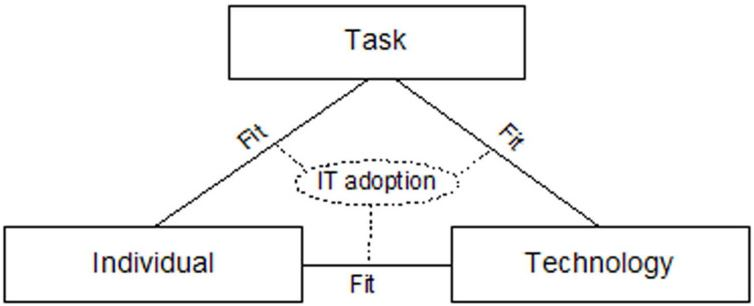
\includegraphics[scale=0.5]{FITT.jpg}
\caption{FITT-arkitekturen}
\label{FITT-arkitekturen}
\end{figure}

\noindent
En $"$bruker$"$ kan her representere både en enkelt bruker, eller en brukergruppe. $"$Teknologi$"$ inkluderer både tekniske verktøy som programmvare, maskinvare og nettverket, og andre verktøy som er nødvendig for utførelsen av en oppgave, som papirbaserte verktøy. $"$Oppgave$"$ er helheten av oppgaver og arbeidsprosesser som må utføres av brukeren med den gitte teknologien. $"$Organisasjon$"$ blir ikke behandlet som et eget objekt i denne sammenhengen, men kan sees som en del av enten bruker-objektet (i betydningen at brukerene jobber i forskjellige roller og grupper i en organisasjon) eller oppgave-objektet (i betydningen at oppgavene og prosessene er organisert på en gitt måte).

\noindent
Med denne tilnærmingen kan vi nå definere målet med IT-ledelse som de å finne en optimal tilpassning (fit) mellom bruker, oppgave og teknologi.
Hvert av disse objektene har en rekke egenskaper, og tilpassningens kvalitet (quality of fit) avhenger av disse, og hvorvidt og i hvilken grad de er tilstede. Listen under nevner noen av egenskapene hver av objektene kan inneha (listen er ikke en fullstendig oversikt). 

\begin{itemize}
\item Brukere: IT-kunnskap, motivasjon og interesse for oppgaven som skal utføres, fleksibilitet og åpenhet for endringer i arbeidsmåte, team-kultur, organisatorisk kontekst, sammarbeidet innenfor team og politikk innen en organisasjon
\item Oppgave: organisering av oppgavene som skal gjennomføres, gjensidig avhengighet mellom oppgavene og oppgavenes grad av kompleksitet
\item Teknologi: stabilitet og brukbarhet ved et program- eller maskinvare-verktøy, verktøyets kostnad, funksjonalitet, tilgjengelig teknisk infrastruktur, integrasjon av verktøy og verktøy tilgjengelig i en gitt klinisk situasjon
\end{itemize}

\noindent
Dersom sammensettnignen av disse egenskapene ikke er optimal, kan man direkte påvirke egenskapene til de enkelte objektene. Et eksempel på dette kan være å gi de ansatte opplæring i systemet, og dermed øke tilstedeværelsen av egenskapen IT-kunnskap hos objektet brukerene. Da dette er tiltak som påvirker objektene direkte, vil vi kunen si at det er en indirekte påvirkning på samspillet mellom objektene.
Det vil alltid finnes eksterne faktorer som er vanskeligere eller umulig å påvirke, som høy utskiftning av stab, eller nye lover og regler. disse eksterne faktorene fører til at det aldri vil oppstå et statisk situasjon med hensyn på de tre dimensjonene av samspill. 

\noindent
Ved å bruke dette rammeverket kan man lettere se hvor eventuelle problemer ved innføringen ligger. En vanlig feiltolkning er at problemer som ligger i smaspillet mellom brukerene og oppgaven blir tillagt teknologien. Et eksempel på dette er dersom innføringen av et nytt IT-system gir brukerene en større mengde dokumentasjonsoppgaver. Ofte vil det nye systemet (teknologien) få skylden for dette, mens problemet ligger i brukerens misnøye med oppgaven, og ikke har noe med teknologien å gjøre.

